\documentclass{standalone}

\usepackage{tikz}
\usetikzlibrary{shapes.geometric, arrows}

\tikzstyle{start} = [rectangle, rounded corners, minimum width=2cm, minimum height=1cm,text centered, draw=black, fill=red!30]
\tikzstyle{stop} = [rectangle, rounded corners, minimum width=2cm, minimum height=1cm,text centered, draw=black, fill=blue!30]

\tikzstyle{io} = [trapezium, trapezium left angle=70, trapezium right angle=110, minimum width=2cm, minimum height=1cm, text centered, draw=black, fill=blue!30]
\tikzstyle{process} = [rectangle, minimum width=2cm, minimum height=1cm, text centered, draw=black, fill=orange!30]
\tikzstyle{classifier} = [rectangle, minimum width=2cm, minimum height=1cm, text centered, draw=black, fill=green!30]
\tikzstyle{decision} = [diamond, minimum width=2cm, minimum height=1cm, text centered, draw=black, fill=green!30]

\tikzstyle{arrow} = [thick,->,>=stealth]

\begin{document}
	
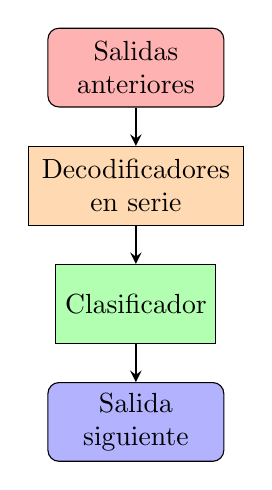
\begin{tikzpicture}[node distance=1.5cm]
\node (start) [start, text width=2cm] {Salidas anteriores};
%\node (enc) [process, below of=start] {Codificador};
\node (dec) [process, below of=start, text width=2.5cm] {Decodificadores en serie};
%\node (outs) [startstop, left of=dec, xshift=-1.3cm, text width=2cm] {Salidas anteriores};
\node (clas) [classifier, below of=dec] {Clasificador};

\node (out) [stop, below of=clas, text width=2cm] {Salida siguiente};

%\node (pro1) [process, below of=in1] {Process 1};
%\node (dec1) [decision, below of=pro1, yshift=-0.5cm] {Decision 1};

\draw [arrow, yshift=1cm] (start) -- (dec);
%\draw [arrow] (enc) -- (dec);
\draw [arrow] (dec) -- (clas);
\draw [arrow] (clas) -- (out);

%\draw [arrow] (outs) -- (dec);

%\draw [arrow] (in1) -- (pro1);
%\draw [arrow] (pro1) -- (dec1);


\end{tikzpicture}

\end{document}